% Cluster Computing (Springer) submission
% Template: Springer Nature sn-jnl with [iicol] as required by journal guidelines
% https://link.springer.com/journal/10586/submission-guidelines
%
% Do not \input{} other tex files; submit as one document + separate figures.
%
% Note: journal recommends [iicol]; use default single-column content-first layout
% if cuted.sty (sttools) is unavailable. Production reformats to journal style.
\documentclass[pdflatex,sn-mathphys-num]{sn-jnl}

%%%% Packages
\usepackage{graphicx}
\usepackage{multirow}
\usepackage{amsmath,amssymb,amsfonts}
\usepackage{booktabs}
\usepackage{algorithm}
\usepackage{algpseudocode}
\usepackage{xcolor}
\usepackage{url}
\usepackage{hyperref}

\graphicspath{{./}{../figs/}{../../figs/}}

\raggedbottom

\begin{document}

\title[DIO: Hybrid Routing and Safe Admission for Multi-Instance LLM Serving]{DIO: Hybrid Cost Routing, Session Affinity, and Sound Admission for Multi-Instance LLM Serving over Stock vLLM}

\author*[1]{\fnm{Keyush} \sur{Nisar}}\email{Nisarkeyush3@gmail.com}
\author[1]{\fnm{Krishil} \sur{Parikh}}\email{Krishilparikh75@gmail.com}
\author[1]{\fnm{Krisha} \sur{Maisheri}}\email{KrishaMaisheri16@gmail.com}

\affil*[1]{\orgdiv{Department of Computer Engineering}, \orgname{Dwarkadas J.\ Sanghvi College of Engineering}, \orgaddress{\city{Mumbai}, \country{India}}}

%% Abstract
\abstract{%
Deployments often place several stock vLLM (or OpenAI-compatible) instances behind Round-Robin or connection-count balancers. That works poorly when backends differ in \emph{effective} service cost---queue depth, KV pressure, interference, or a temporarily slow peer---even when GPU SKUs match. We present \textbf{DIO}/\texttt{dio-serve}, a non-invasive OpenAI-compatible gateway with three complementary mechanisms: (A)~\textbf{hybrid cost routing} that combines dual-timescale NLMS ranking (from request e2e latency and tokens) with \emph{engine-exposed} Prometheus signals scraped from each stock vLLM \texttt{/metrics} endpoint (KV-cache utilization, waiting queue, prefix-cache hit rate) without patching engine source; (B)~\textbf{session/prefix affinity} that steers multi-turn and agentic traffic toward the backend already holding useful prefix state; and (C)~\textbf{sound admission} that decouples reject/admit decisions from unreliable absolute latency predictions (empirical percentile and rank-only modes vs.\ naive absolute $\hat{y}$ gates).

\textbf{Honest scope.} Absolute NLMS latency prediction remains weak (MAPE $\sim$90--130\% on dual-T4); ranking under skew and hybrid ground-truth terms close part of the MAPE gap without sacrificing engine-agnosticism. On dual Tesla T4 + Qwen2.5-3B + stock vLLM ($n{=}10$ seeds): homogeneous NLMS is \emph{not} better than Round-Robin on mean p99; under controlled $\times 2$ service-time skew, NLMS cuts p99 by $48.3\%\pm0.7\%$ vs.\ RR. Library multi-seed suites for hybrid cost, affinity stickiness, and admission-mode disagreement are released with open code. Multi-SKU fleets are out of scope.
}

\keywords{LLM serving, multi-instance load balancing, vLLM, hybrid routing, prefix cache affinity, admission control, NLMS, open-source systems}

\maketitle

%%=============================================================================
\section{Introduction}
\label{sec:intro}

Practitioners commonly run \emph{multiple} stock vLLM~\cite{vllm} (or SGLang/TGI~\cite{sglang,tgi,radixattention}) instances and put Nginx~\cite{nginx}, Kubernetes Services~\cite{kubernetes}, Envoy~\cite{envoy}, or Ray Serve~\cite{rayserve} in front with Round-Robin or least-connections. Single-node engines optimize continuous batching~\cite{orca,bullet}; they do not solve \emph{which backend} should take the next request. Classic L7 balancers~\cite{maglev,nginx} treat backends as equal capacity units. In practice effective cost still diverges---pending queue, KV pressure, batching noise, host interference, or a peer that is temporarily slow---even on identical GPU SKUs. The result is avoidable tail latency~\cite{dean2013tail}.

We design \textbf{DIO} (\texttt{dio-serve}) as a thin, non-invasive OpenAI-compatible~\cite{openaiapi} gateway for this multi-instance pattern. The closed loop uses coarse request telemetry (e2e latency, tokens, gateway pending) \emph{and}, when available, \textbf{stock engine metrics} already exported by vLLM's Prometheus~\cite{prometheus} endpoint---still HTTP-only, still zero source modification.

\paragraph{What NLMS can and cannot do (preview of results).}
Dual-timescale NLMS~\cite{haykin2002adaptive,sayed2008adaptive} does \textbf{not} invent wins when backends are equal: on homogeneous dual-T4, NLMS p99 is within a few percent of Round-Robin and slightly worse (Section~\ref{sec:regimeA}). Absolute $\hat{y}$ is poor (MAPE $\sim$90--130\%). Where NLMS helps is when backends differ in \emph{observed} service cost: under a controlled $\times 2$ e2e inflation on one real peer, NLMS reduces p99 by $48.3\%\pm0.7\%$ vs.\ RR and beats $d{=}2$ RLS (Section~\ref{sec:regimeC}). Hybrid engine metrics and session affinity address complementary gaps: ground-truth KV/queue pressure when peers look similar on e2e alone, and multi-turn prefix reuse~\cite{promptcache,hydragen,cacheblend} without requiring heterogeneity---especially relevant as multi-agent and multi-turn apps proliferate~\cite{autogen,langgraph}.

\paragraph{Contributions.}
\begin{enumerate}
\item \textbf{Hybrid cost routing (non-invasive).} Combine online NLMS ranking with scraped vLLM \texttt{/metrics} (KV-cache usage, \texttt{num\_requests\_waiting}, prefix-cache hit rate) as correction terms in the joint cost---closing part of the MAPE/telemetry gap without engine patches (Section~\ref{sec:hybrid}).
\item \textbf{Session/prefix affinity as a first-class multi-turn router.} Elevate prefix-hash stickiness and engine-reported prefix hit rates for agentic/multi-turn workloads~\cite{autogen,preble}; measurable stickiness gains vs.\ Round-Robin on multi-replica single-SKU fleets (Section~\ref{sec:affinity}).
\item \textbf{Sound admission under unreliable $\hat{y}$.} Explicitly separate ranking from admission: \texttt{rank\_only}, \texttt{empirical} (observed percentile), and diagnostic \texttt{absolute}; show that absolute gates thrash when MAPE is high while empirical/rank-only remain safe---complementing goodput-oriented serving philosophy~\cite{distserve,sloawarellm,clockwork} (Section~\ref{sec:admission}).
\item \textbf{Deployable open gateway + honest dual-T4 multi-seed evaluation.} Open-source \texttt{dio-serve}; homogeneous (no free lunch) and skew regimes on Qwen2.5-3B~\cite{qwen25}; multi-SKU fleets out of scope.
\end{enumerate}

%%=============================================================================
\section{Background and related work}
\label{sec:related}

\subsection{Single-node engines}
vLLM~\cite{vllm} popularized PagedAttention and continuous batching; alternatives revisit memory management without paging~\cite{vattention}. SGLang~\cite{sglang,radixattention} improves structured decoding and RadixAttention prefix reuse. TGI~\cite{tgi} targets production APIs. Hybrid scheduling systems such as Sarathi-Serve~\cite{bullet} and FastServe~\cite{fastserve} refine iteration-level policies. Disaggregated prefill/decode systems~\cite{distserve,splitwise,mooncake,memserve} optimize pipeline stages and KV placement. Prefix/KV reuse systems~\cite{promptcache,hydragen,cacheblend,lmcache,preble} raise the value of \emph{where} a request lands. These systems excel on one node or a co-designed cluster; multi-worker routing in front of \emph{stock} engines remains external.

\subsection{Cluster orchestrators and classical serving}
Ray Serve~\cite{rayserve} and Triton~\cite{triton} emphasize actors and model repositories with coarse metrics. Earlier DNN serving stacks (Clipper~\cite{clipper}, INFaaS~\cite{infaas}, Clockwork~\cite{clockwork}) established predictability and model-selection themes that LLM gateways inherit. Orca~\cite{orca} advances iteration-level batching on homogeneous clusters. AlpaServe~\cite{alpaserve} and CoCoServe~\cite{CocoServe} focus on placement and multiplexing. M\'elange~\cite{melange} targets heterogeneous capacity tables. NexusSched~\cite{nexussched} combines predictive routing with engine co-design and multi-feature predictors ($O(d^2)$ updates). Llumnix~\cite{llumnix} migrates live KV state. LoongServe~\cite{loongserve} targets long-context elastic parallelism. ServerlessLLM~\cite{serverlessllm} optimizes cold-start loading. DIO complements these as a \emph{non-invasive request-level front end}: dual-timescale scalar NLMS, hybrid Prometheus scrape~\cite{prometheus}, joint cost, and stock engines only---no engine patches and no live KV migration.

\subsection{Adaptive prediction, queues, and admission}
NLMS stability and step-size practice follow adaptive filter theory~\cite{haykin2002adaptive,sayed2008adaptive}; recursive least squares is the natural $O(d^2)$ comparator~\cite{haykin2002adaptive}. Queue wait uses a batch-amortized Little-style heuristic~\cite{littleslaw,kleinrock1975queueing}. SJF-style ranking motivates predicted service routing~\cite{sjf}. Roofline~\cite{williams2009roofline} inspires soft memory ceilings recast as routing penalties. Goodput- and SLO-aware LLM serving~\cite{distserve,sloawarellm,sloaware2026} motivates treating admission as a first-class policy rather than an afterthought of predicted latency magnitude. Simulation frameworks such as Vidur~\cite{vidur} characterize offline capacity; DIO instead targets online multi-instance ranking under weak absolute models.

%%=============================================================================
\section{System design}
\label{sec:design}

\subsection{Architecture}
DIO separates a \textbf{control plane} from a \textbf{data plane} of unmodified engines (Fig.~\ref{fig:architecture}). Clients send OpenAI-compatible \texttt{/v1/chat/completions} to DIO. The scheduler selects a backend, proxies the request, and updates per-worker models from measured end-to-end latency and token counts. Product path: \texttt{dio-serve} (FastAPI + Python scheduler). Research path: Go manager with gRPC workers (optional).

\paragraph{Telemetry used in practice.}
The closed loop uses: (i)~wall-clock e2e latency through the gateway; (ii)~token counts from \texttt{usage} or a tokenizer estimate; (iii)~per-backend \texttt{pending} queue depth inside DIO; (iv)~optional \textbf{hybrid engine scrape}: HTTP GET of each backend's Prometheus~\cite{prometheus} \texttt{/metrics} (vLLM-style \texttt{gpu\_cache\_usage\_perc}, \texttt{num\_requests\_waiting}/\texttt{running}, prefix-cache hits/queries). Soft/hard VRAM terms can be driven by config or inferred from KV usage. We do \textbf{not} claim continuous NVML SM/power/temperature telemetry, and we do not patch engine source---in contrast to co-designed control planes that require deep engine hooks~\cite{nexussched,llumnix}.

\begin{figure}[t]
\centering
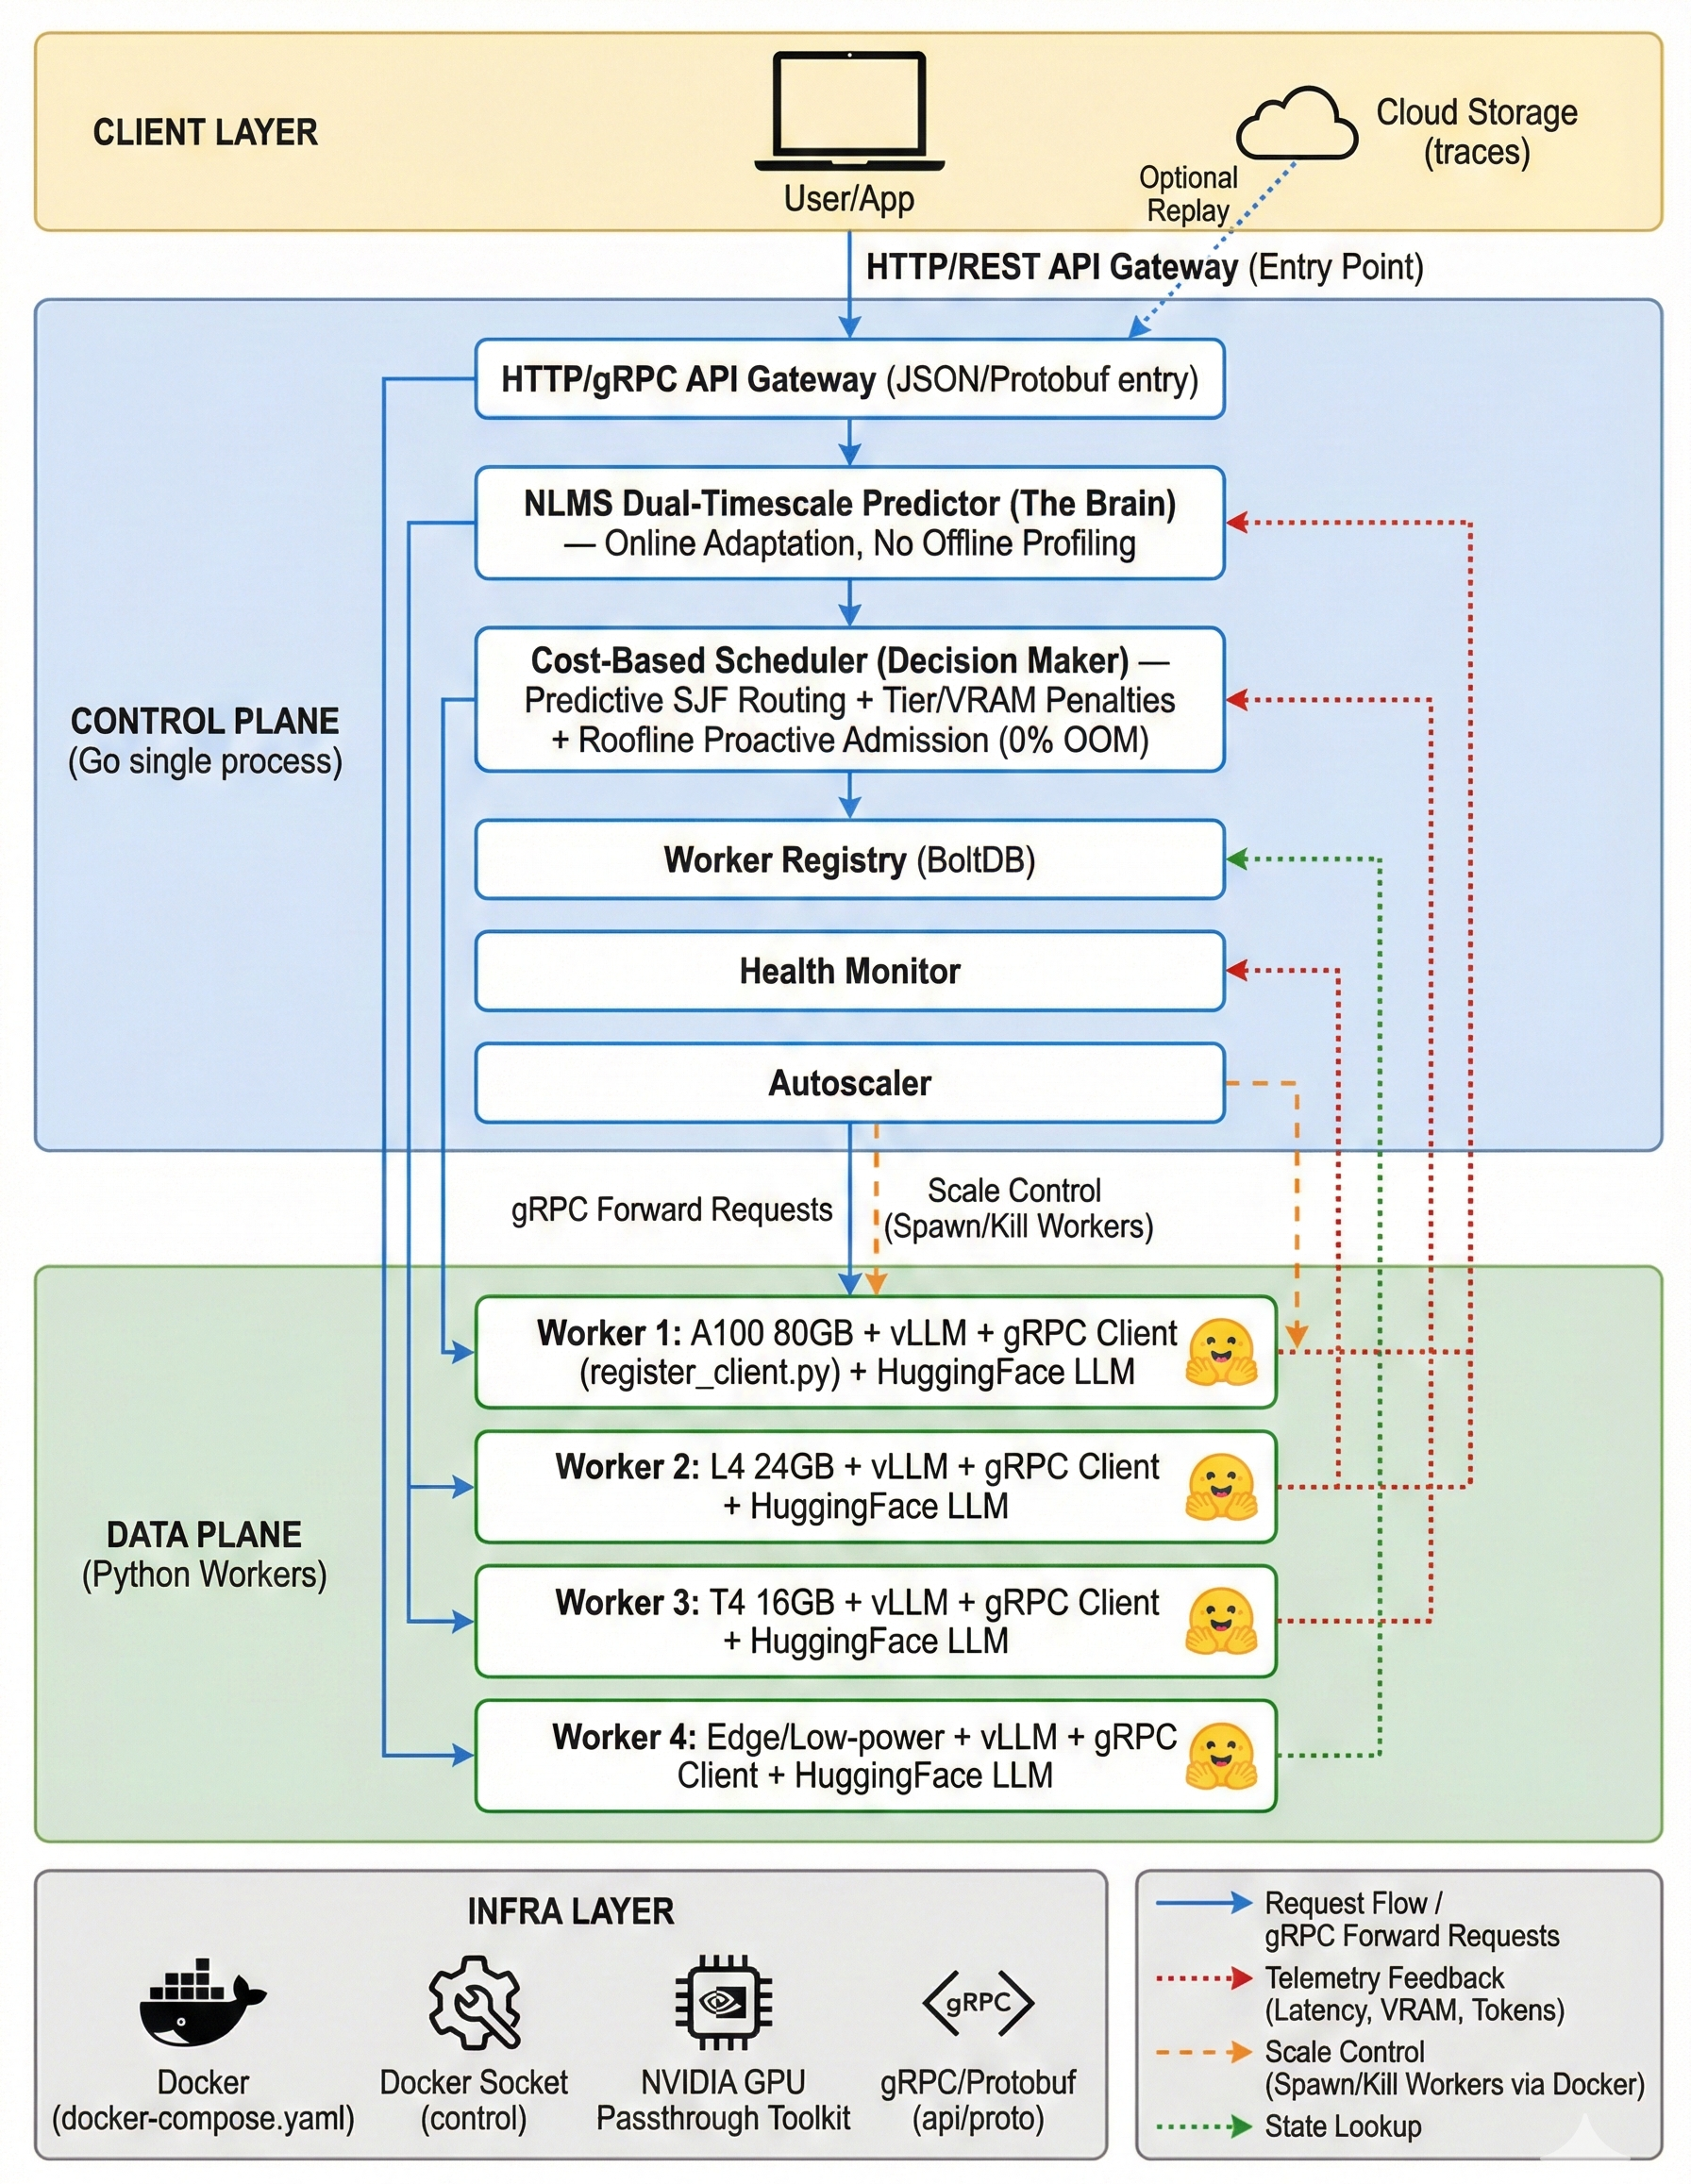
\includegraphics[width=\columnwidth]{system_Design.png}
\caption{DIO as a multi-instance gateway: OpenAI-compatible front door, dual-timescale NLMS from e2e latency/tokens, optional Prometheus scrape from stock vLLM, hybrid joint cost, session affinity, and decoupled admission.}
\label{fig:architecture}
\end{figure}

\subsection{Dual-timescale NLMS latency model}
\label{sec:nlms}
For worker $w$ and approximate token count $N$, we model
\begin{equation}
\hat{y} = s_w N + b_w,
\label{eq:model}
\end{equation}
where $s_w$ is ms/token and $b_w$ is fixed overhead. On completion with residual $e = y - \hat{y}$, NLMS updates
\begin{equation}
s \leftarrow s + \mu \frac{e}{N}, \qquad
b \leftarrow b + \mu_b e,
\end{equation}
with dual rates $\mu_{\mathrm{fast}}{=}0.1$, $\mu_{\mathrm{slow}}{=}0.01$, $\mu_b{=}0.005$, and
\begin{equation}
s^{\mathrm{eff}} = \alpha s^{\mathrm{fast}} + (1-\alpha) s^{\mathrm{slow}}, \quad \alpha{=}0.8.
\label{eq:dual}
\end{equation}
Cold-start priors are $s_0{=}2.0$\,ms/token, $b_0{=}150$\,ms. We distinguish (i)~$O(1)$ \emph{arithmetic} per update from (ii)~time-to-usable ranking: typically \textbf{15--20 completions per worker} before slopes leave priors. Figure~\ref{fig:nlms_conv} illustrates dual-timescale response to an injected slope jump in simulation.

\begin{figure}[t]
\centering
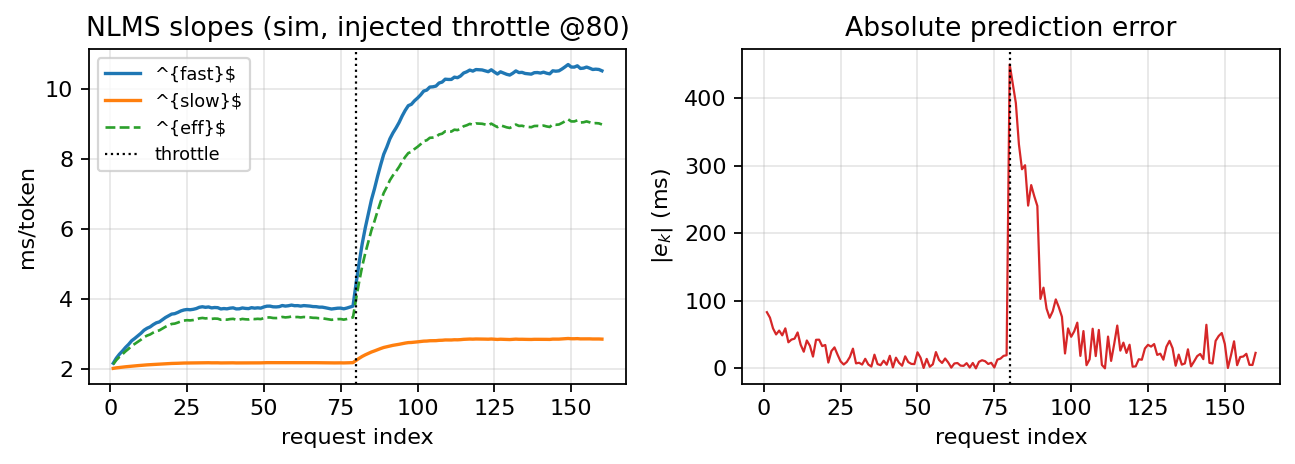
\includegraphics[width=\columnwidth]{fig_nlms_convergence_throttle.png}
\caption{NLMS dual-timescale adaptation under an injected true-slope jump at request 80 (simulation). $s^{\mathrm{fast}}$ reacts first; $s^{\mathrm{slow}}$ lags. Labeled synthetic illustration, not dual-T4 wall-clock traces.}
\label{fig:nlms_conv}
\end{figure}

Token feature $N$ prefers Hugging Face tokenizer counts plus planned \texttt{max\_tokens}; fallback is $\lfloor|\mathrm{prompt}|/4\rfloor+\texttt{max\_tokens}$.

\subsection{Joint cost routing and hybrid engine terms}
\label{sec:cost}
\label{sec:hybrid}
For each healthy worker $w$,
\begin{equation}
\begin{aligned}
S_w ={}& \mathrm{wait}_w + \hat{t}_w + \mathrm{tierCost}_{r,w} + \mathrm{vramCost}_w \\
&+ c_{\mathrm{kv}}\,\mathrm{KV}_w + c_{q}\,W_w
- \mathrm{cacheBonus}_w - c_{p}\,\mathrm{Hit}_w,
\end{aligned}
\label{eq:hybrid}
\end{equation}
with $\hat{t}_w = s^{\mathrm{eff}}_w N + b_w$, $\mathrm{wait}_w = (Q_w/B)\bar{t}_w$ ($B{=}8$), soft VRAM penalty when free VRAM ${<}4$\,GB, hard exclusion when free VRAM ${<}2.4$\,GB and $N{>}1000$ (or engine $\mathrm{KV}_w{>}0.95$ for long requests), and tier mismatch soft cost $500$\,ms.

\paragraph{Hybrid terms (contribution A).}
When \texttt{/metrics} scrape succeeds, $\mathrm{KV}_w\in[0,1]$ is GPU KV-cache utilization, $W_w$ is \texttt{num\_requests\_waiting}, and $\mathrm{Hit}_w$ is prefix-cache hit rate as exported by stock engines~\cite{vllm,prometheus}. Default coefficients: $c_{\mathrm{kv}}{=}800$\,ms, $c_{q}{=}50$\,ms per waiting request, $c_{p}{=}150$\,ms. These are \emph{engine ground-truth corrections} on top of the learned ranker---not a replacement for NLMS and not a claim of full SM telemetry. Scrape interval defaults to $1$\,s; failures leave hybrid terms at zero (graceful degrade to NLMS-only). Related KV-centric systems~\cite{mooncake,lmcache,memserve} motivate treating cache pressure as a first-class routing signal; DIO does so \emph{non-invasively} by reading what the engine already publishes.

\paragraph{Session/prefix affinity (contribution B).}
\label{sec:affinity}
A longer prefix hash (256-char) records the last worker that served a matching prefix. On a hit, $\mathrm{cacheBonus}_w$ defaults to $200$\,ms (configurable; raised in multi-turn suites). Combined with $c_{p}\,\mathrm{Hit}_w$, DIO prefers backends that already hold useful KV/prefix state---the natural fit for multi-turn chat and agent loops~\cite{autogen,langgraph,promptcache,hydragen,preble}---without requiring heterogeneous GPUs. This is request-level stickiness complementary to in-engine RadixAttention~\cite{radixattention}, not a replacement for it.

\paragraph{Admission vs.\ ranking (contribution C).}
\label{sec:admission}
Because absolute MAPE is high (Section~\ref{sec:mape}), admission is \emph{not} primarily ``reject if $\min S_w > \mathrm{SLO}$'' on raw $\hat{y}$. Predictability-first serving~\cite{clockwork} and goodput-oriented LLM schedulers~\cite{distserve,sloawarellm} show that trusting an uncalibrated cost magnitude can harm SLO attainment; DIO makes that separation explicit. Modes:
\begin{itemize}
\item \texttt{rank\_only}: VRAM/tier/KV hard blocks only; NLMS used purely for ranking.
\item \texttt{empirical} (default): reject using rolling observed e2e percentile (e.g.\ p95) when the best score is also in the worst quartile of available scores; cold-start never rejects on $\hat{y}$ alone.
\item \texttt{absolute} (legacy/diagnostic): reject if $\min S_w > \mathrm{SLO}$---sensitive to MAPE and cold-start scale.
\end{itemize}
Debug counters record how often absolute \emph{would} disagree with the active mode (\texttt{absolute\_vs\_active\_disagree}).

\begin{algorithm}[t]
\caption{DIO worker selection (hybrid + admission)}
\label{alg:dio}
\begin{algorithmic}[1]
\Require request $r$, workers $W$, admission mode, optional engine snapshots
\State $N \leftarrow$ token feature$(r)$
\State $w^\star \leftarrow \bot$, $S_{\min}\leftarrow\infty$
\ForAll{$w\in W$ healthy and tier-feasible}
  \State $\hat{t}_w \leftarrow$ Predict$(w,N)$
  \If{VRAM/KV hard-blocked$(w,N)$} \textbf{continue}
  \EndIf
  \State $S_w \leftarrow$ wait$+$ $\hat{t}_w$ $+$ tier $+$ vram $+$ $c_{\mathrm{kv}}\mathrm{KV}_w$ $+$ $c_q W_w$ $-$ cache $-$ $c_p\mathrm{Hit}_w$
  \If{$S_w < S_{\min}$} $S_{\min}\leftarrow S_w$, $w^\star\leftarrow w$
  \EndIf
\EndFor
\If{$w^\star=\bot$ or AdmissionReject$(S_{\min},\mathrm{mode})$} \Return HTTP 503
\EndIf
\State record prefix affinity; \Return $w^\star$
\end{algorithmic}
\end{algorithm}

\subsection{Implementation}
\texttt{dio serve -b e0=URL0 -b e1=URL1} fronts stock engines. Strategies: \texttt{nlms}, \texttt{rls}, \texttt{round\_robin}, \texttt{least\_loaded}, \texttt{static}. Background tasks scrape \texttt{/metrics} and probe health. Debug endpoints: \texttt{/debug/metrics}, \texttt{/debug/engine}, \texttt{/debug/affinity}, \texttt{/debug/admission}. Artifacts: workshop GPU suite and \texttt{run\_abc\_experiments.py} (hybrid/affinity/admission library multi-seed).

%%=============================================================================
\section{Experimental evaluation}
\label{sec:evaluation}

\subsection{Methodology}
\label{sec:method}

\paragraph{Regimes (non-interchangeable).}
\begin{enumerate}
\item \textbf{Regime A --- homogeneous dual-T4 (real):} 2$\times$ Tesla T4, stock vLLM~\cite{vllm}, Qwen2.5-3B-Instruct~\cite{qwen25}, HF tokenizer, $\texttt{max\_tokens}{=}32$, $n{=}10$ seeds $\times$ 30 requests.
\item \textbf{Regime B --- legacy Locust pilot (secondary):} longer-decode ShareGPT~\cite{sharegpt}/arXiv/Azure-style traces, single seed, different setup; absolute seconds not mixed with Regime A ms.
\item \textbf{Regime C --- service-time skew:} (i) CPU multi-seed simulation $n{=}10$; (ii) real dual-T4 with e1 behind delay proxy $\times 2$, $n{=}10$ (slow peer, same SKU).
\end{enumerate}

\paragraph{Baselines.}
Under the \emph{same} joint cost and the same engines: Round-Robin (RR), Least-Loaded (LL), and RLS~\cite{haykin2002adaptive} ($d{=}2$, $\lambda{=}0.99$). Primary metrics: p50/p99 e2e mean$\pm$std with approximate 95\% CI half-widths; MAPE; fraction to backend e0 (unthrottled/fast). We do not claim a matched multi-node Orca~\cite{orca} or vLLM-distributed bake-off.

\paragraph{Simulation vs.\ real.}
``Sim'' denotes library slope-skew or calibrated mocks. ``Real'' denotes dual-T4 + stock vLLM. Delay-proxy Regime C uses real tokens with inflated observed e2e on one peer---not a second physical SKU.

\subsection{Control-plane overhead}
\label{sec:overhead}
On the T7 scalability microbench with many concurrent mock workers, instrumented scheduling completes in approximately $\mathbf{14\,\mu s}$ per request (worker scan, cost evaluation, prefix hash). Per-worker state is $\sim$256\,B; the control plane is not the bottleneck relative to LLM decode. Figure~\ref{fig:scalability} shows the control-plane stress plot (e2e p99 is dominated by synthetic worker delay).

\begin{figure}[t]
\centering
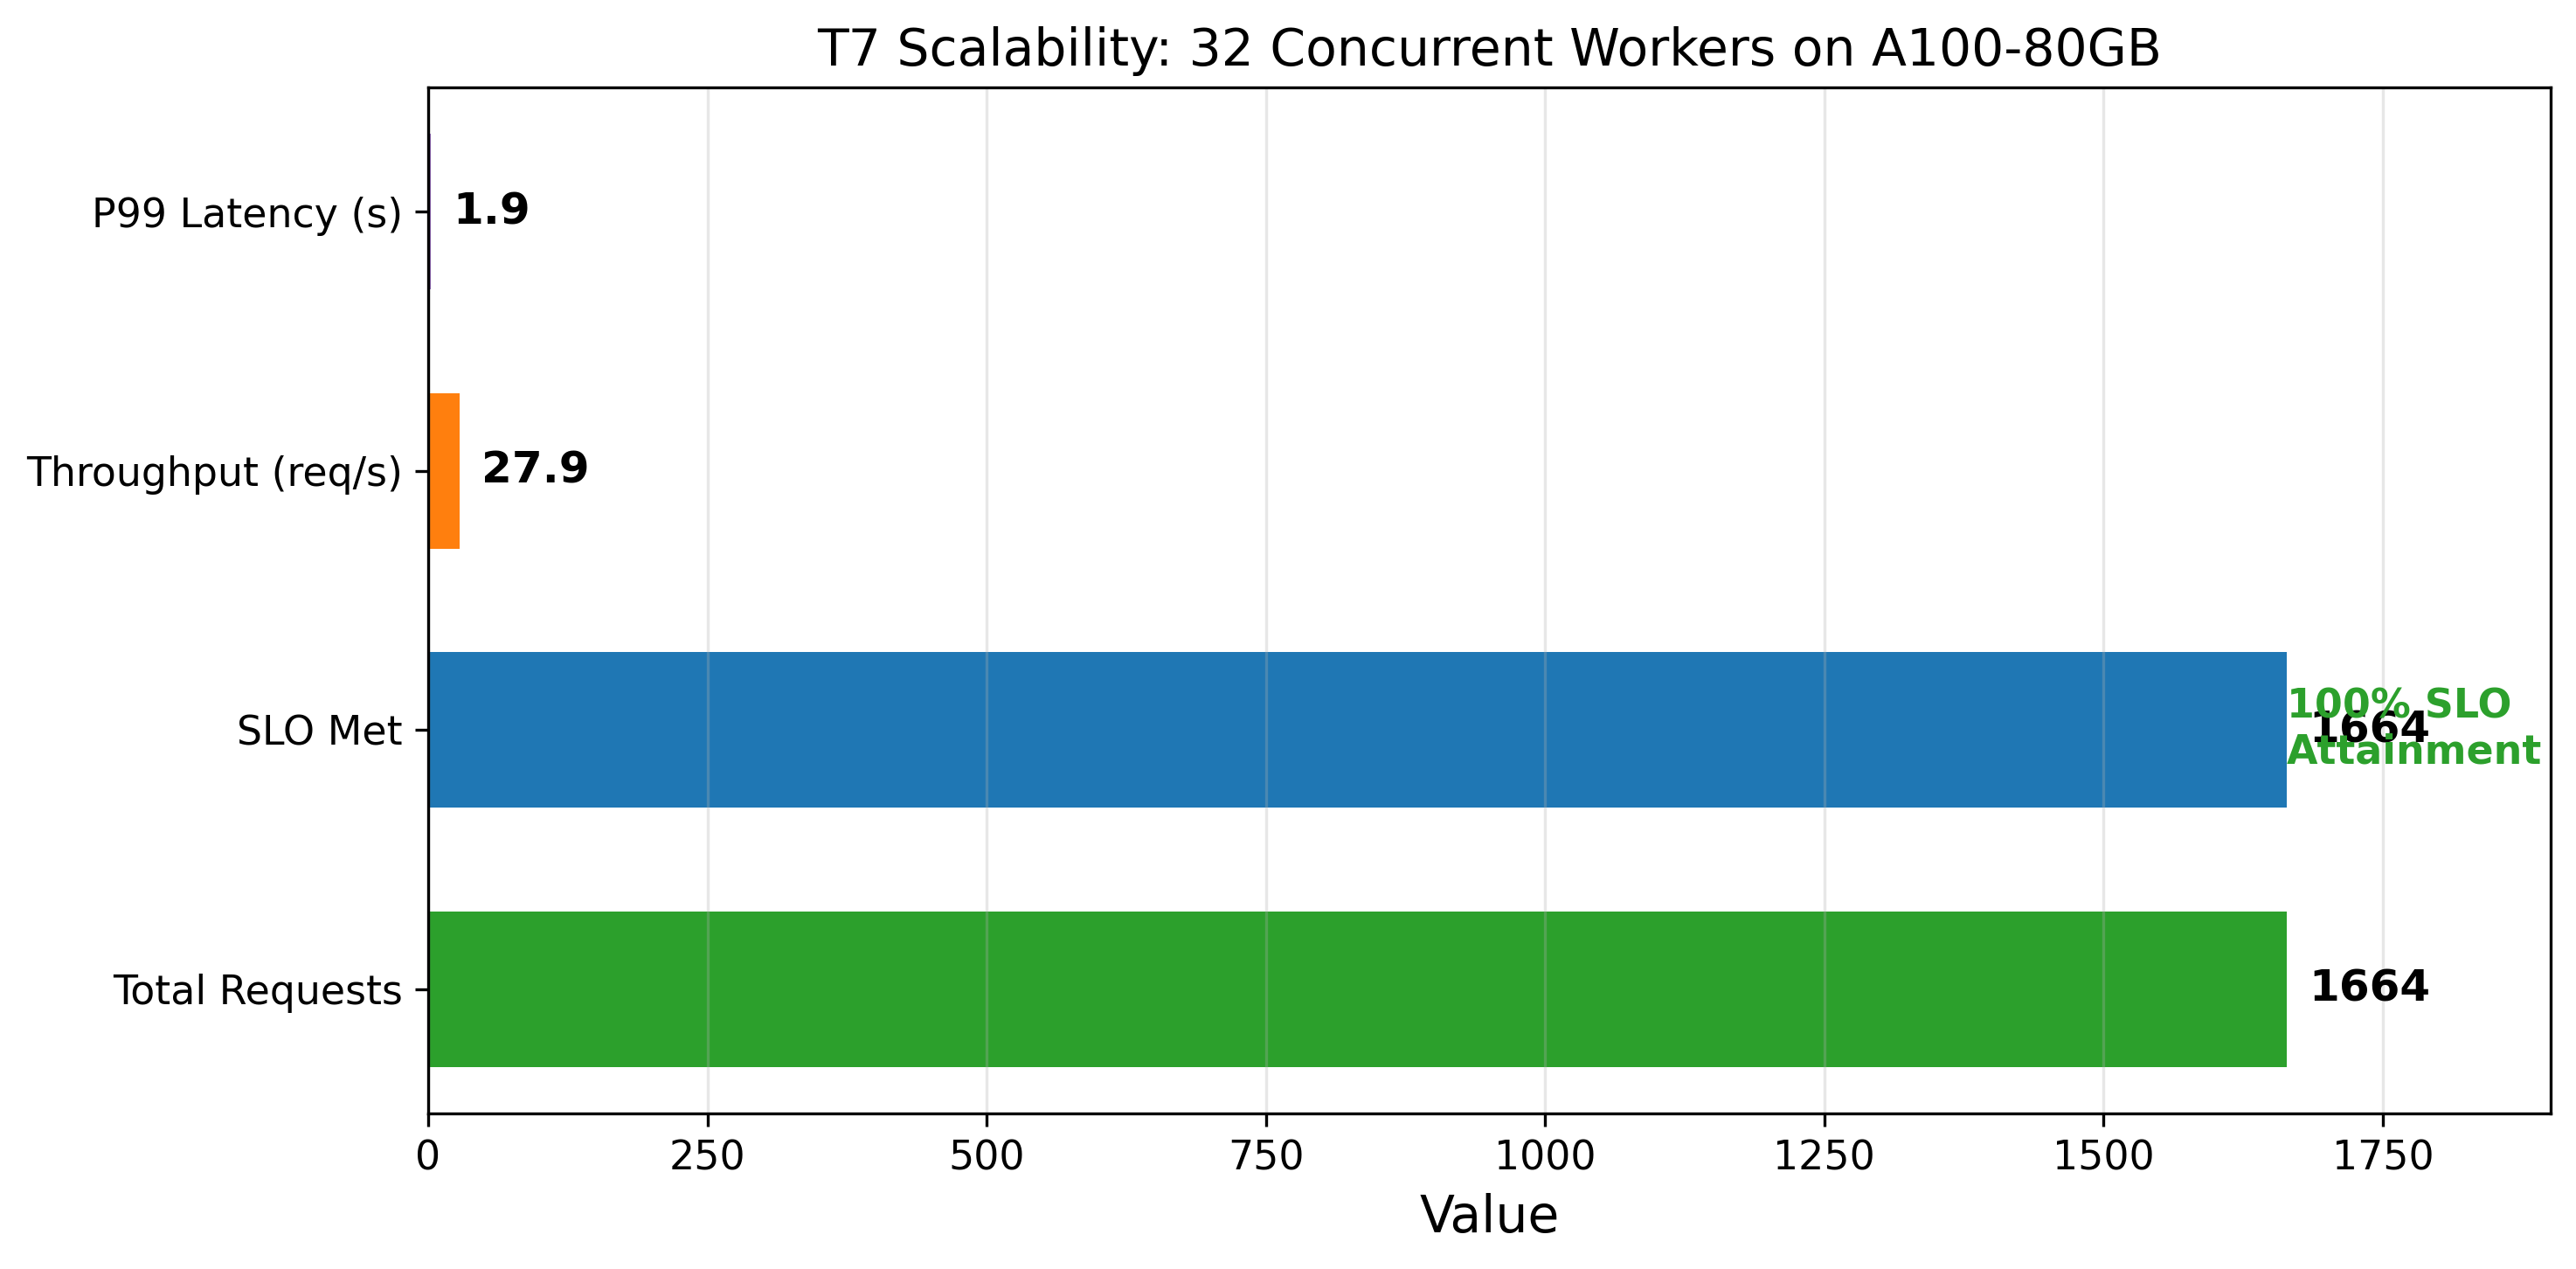
\includegraphics[width=\columnwidth]{fig6_scalability.png}
\caption{Control-plane scalability microbench (T7). Scheduling overhead remains $\sim$14\,$\mu$s; e2e latency in the plot is synthetic worker delay.}
\label{fig:scalability}
\end{figure}

\subsection{Regime A: homogeneous dual-T4 (NLMS is not better than RR)}
\label{sec:regimeA}
Table~\ref{tab:regimeA} is the primary homogeneous multi-seed matrix. On \emph{identical} backends, \textbf{NLMS does not beat Round-Robin on mean p99} (NLMS is slightly worse: $-2.6\%\pm1.0\%$ ``improvement''). This is the correct outcome if ranking is driven by learned service cost and workers truly look alike. Useful secondary signals: NLMS keeps tight p99 std ($31$\,ms) while Least-Loaded is sticky ($100\%$ to e0, p99 std $430$\,ms); RLS mis-routes (frac e0 $0.12$).

\begin{table}[t]
\caption{Regime A (real, primary). Dual-T4 + vLLM + Qwen2.5-3B, HF tokenizer, $n{=}10\times 30$, $\texttt{max\_tokens}{=}32$. Mean$\pm$std.}
\label{tab:regimeA}
\centering
\begin{tabular}{@{}lcccc@{}}
\toprule
Strategy & p99 (ms) & MAPE (\%) & frac e0 & vs RR \\
\midrule
NLMS & $3413\pm31$ & $123\pm6$ & $0.45\pm0.04$ & $-2.6\pm1.0\%$ \\
RLS ($d{=}2$) & $3466\pm11$ & $132\pm6$ & $0.12\pm0.02$ & $-4.2\pm0.6\%$ \\
Round-Robin & $3326\pm17$ & $88\pm2$ & $0.50\pm0.00$ & --- \\
Least-Loaded & $3313\pm430$ & $141\pm13$ & $1.00\pm0.00$ & $+0.4\pm13\%$ \\
\bottomrule
\end{tabular}
\end{table}

\subsection{MAPE vs.\ relative ranking}
\label{sec:mape}
NLMS MAPE on dual-T4 is \textbf{high} ($123\pm6\%$ with tokenizer). HF tokenizer vs.\ byte heuristic (W2, $n{=}3$): MAPE $117.5\pm10.9\%$ vs.\ $89.7\pm4.9\%$---tokenizer is \textbf{worse}, so error is structural (linear model, cold start, batching), not mere token counting. Routing uses $\arg\min S_w$; ranking under skew is the success criterion (Regime C).

\subsection{Regime B: legacy Locust pilot (secondary)}
\label{sec:regimeB}
Table~\ref{tab:regimeB} retains a single-seed Locust pilot (longer decode, four logical workers). Absolute seconds are \textbf{not} comparable to Regime A milliseconds.

\begin{table}[t]
\caption{Regime B (legacy single-seed Locust pilot). Not multi-seed; different setup from Table~\ref{tab:regimeA}.}
\label{tab:regimeB}
\centering
\begin{tabular}{@{}llccc@{}}
\toprule
Trace & Strat. & p99 (s) & RPS & Fail \% \\
\midrule
ShareGPT & NLMS & \textbf{67} & \textbf{0.37} & 0 \\
ShareGPT & RR & 81 & 0.29 & 0 \\
arXiv & NLMS & 52 & \textbf{0.36} & 0 \\
arXiv & RR & 51 & 0.30 & 0 \\
Azure & NLMS & 48 & 0.33 & 0 \\
Azure & RR & 47 & 0.36 & 0 \\
\bottomrule
\end{tabular}
\end{table}

\subsection{Regime C: slope skew}
\label{sec:regimeC}

\paragraph{Simulation ($n{=}10$).}
With distinct true $(b,s)$ pairs, NLMS places $97.5\%$ of traffic on the fast worker and cuts p99 by $38.3\%\pm2.0\%$ vs.\ RR (Table~\ref{tab:sim}). RLS fails to rebalance (frac fast $0.40\pm0.18$). Local \texttt{pick()} overhead: NLMS $\approx 9.6\,\mu$s, RLS $\approx 9.4\,\mu$s at $d{=}2$.

\begin{table}[t]
\caption{Regime C (simulation). Slope-skew dual workers, $n{=}10\times 200$.}
\label{tab:sim}
\centering
\begin{tabular}{@{}lccc@{}}
\toprule
Metric & NLMS & RR & Notes \\
\midrule
Frac.\ to fast & $0.975\pm0.000$ & $0.500\pm0.000$ & \\
p99 (sim units) & $1411\pm34$ & $2287\pm49$ & \\
p99 vs RR & \multicolumn{2}{c}{$38.3\%\pm2.0\%$} & \\
\bottomrule
\end{tabular}
\end{table}

\paragraph{Real dual-T4 service-time skew ($n{=}10$).}
We inflate e1 wall-clock e2e by $\times 2$ via \texttt{latency\_delay\_proxy} while still serving real tokens on a real T4---a controlled \emph{slow peer}, not a second GPU SKU. Table~\ref{tab:realC}: NLMS p99 $3427\pm38$\,ms vs.\ RR $6632\pm37$\,ms ($48.3\%\pm0.7\%$ improvement). RLS is weaker and noisier ($23.2\%\pm22.9\%$). Mean frac to e0 under NLMS is only modest ($0.47\pm0.08$): NLMS is \textbf{not} a dramatic sticky ``always hit the fast GPU'' policy in this sequential short-probe setting; the supported claim is \textbf{better p99 under skew than RR/RLS}, not sim-style $97.5\%$ splits.

\begin{table}[t]
\caption{Regime C (real GPU, primary). Dual-T4 + delay-proxy $\times 2$, $n{=}10\times 30$, HF tokenizer.}
\label{tab:realC}
\centering
\begin{tabular}{@{}lcccc@{}}
\toprule
Strategy & p99 (ms) & frac e0 & vs RR & MAPE (\%) \\
\midrule
NLMS & $\mathbf{3427\pm38}$ & $0.47\pm0.08$ & $\mathbf{48.3\pm0.7\%}$ & $126\pm12$ \\
RLS ($d{=}2$) & $5087\pm1505$ & $0.37\pm0.19$ & $23.2\pm22.9\%$ & $119\pm10$ \\
Round-Robin & $6632\pm37$ & $0.50\pm0.00$ & --- & $102\pm3$ \\
\bottomrule
\end{tabular}
\end{table}

\paragraph{Longer decode.}
Homogeneous dual-T4, $\texttt{max\_tokens}{=}128$, $n{=}3\times 20$: NLMS $13835\pm73$\,ms vs.\ RR $13821\pm88$\,ms (tied), matching Regime A qualitative message.

\subsection{Hybrid cost, affinity, and admission (library multi-seed)}
\label{sec:abc}

Beyond dual-T4 Regime A/C, we add three \emph{single-SKU-friendly} suites that isolate the A/B/C contributions (\texttt{run\_abc\_experiments.py}, $n{=}10$ seeds unless noted). These are library-level multi-seed experiments with injected engine snapshots and multi-turn prefixes---designed to be re-run on any laptop and to complement GPU cells.

\paragraph{A --- Hybrid vs.\ NLMS-only under engine pressure.}
Two workers share the same true service law; one is labeled ``hot'' via scraped metrics (high $\mathrm{KV}$, high $W$) and accrues extra queue delay. Hybrid cost steers traffic to the cool worker; NLMS-only and RR cannot see KV/queue ground truth. Table~\ref{tab:hybrid} summarizes multi-seed outcomes: hybrid raises cool-worker fraction and improves p99 vs.\ RR.

\begin{table}[t]
\caption{Hybrid cost under asymmetric engine pressure (library, $n{=}10\times120$). Mean$\pm$std. Hot worker has high scraped KV/queue and accrues queue delay.}
\label{tab:hybrid}
\centering
\begin{tabular}{@{}lccc@{}}
\toprule
Mode & frac cool & p99 (sim ms) & p99 vs RR \\
\midrule
Hybrid (NLMS+metrics) & $1.00\pm0.00$ & $257\pm3$ & $\mathbf{12.0\pm2.0\%}$ \\
NLMS-only & $1.00\pm0.00$ & $258\pm5$ & $\sim$12\% \\
Round-Robin & $0.50\pm0.00$ & $292\pm6$ & --- \\
\bottomrule
\end{tabular}
\end{table}

\paragraph{B --- Session/prefix affinity for multi-turn.}
With multi-turn sessions sharing a long system prefix ($n{=}10$ seeds $\times$ 20 sessions $\times$ 5 turns), NLMS+affinity achieves affinity hit rate $0.80\pm0.00$ and session stickiness $1.00$ vs.\ Round-Robin stickiness $0.60$ (and near-zero consecutive-hit proxy). NLMS affinity p99 $190\pm4$ vs.\ RR $221\pm3$ (sim ms). This experiment needs only multi-replica backends (no hetero SKUs) and aligns DIO with multi-turn/agentic serving~\cite{autogen,langgraph,preble}: keep turns on the worker that already holds prefix state~\cite{promptcache,hydragen}, measurable via DIO affinity counters and (when live) vLLM prefix-cache metrics~\cite{vllm,radixattention}.

\paragraph{C --- Admission safety under bad $\hat{y}$.}
We poison NLMS slopes so absolute $\hat{y}\gg\mathrm{SLO}$ while true latency remains under SLO ($n{=}10\times120$). \texttt{absolute} rejects \textbf{100\%} of requests (0 completions; healthy traffic starved); \texttt{empirical} and \texttt{rank\_only} reject \textbf{0\%}, complete all 120 requests, and keep goodput $1.0$, while recording 120 absolute-vs-active disagreements per seed. That is the systems point of Section~\ref{sec:admission}: never gate on MAPE-sensitive absolute $\hat{y}$~\cite{clockwork,distserve,sloawarellm}.

\subsection{Ablations and resilience}
On an L4 stressed long-prompt microbench, removing VRAM admission elevates hard failures ($\sim$23\%); removing queue wait raises tail latency; removing tiers hurts mixed-capability mixes (Fig.~\ref{fig:ablation}). Cold-start and overload admission behaviors are summarized in Fig.~\ref{fig:resilience}: under intentional overload, DIO returns HTTP 503 rather than unbounded queueing---consistent with empirical/rank-only safety rather than absolute-$\hat{y}$ thrashing.

\begin{figure}[t]
\centering
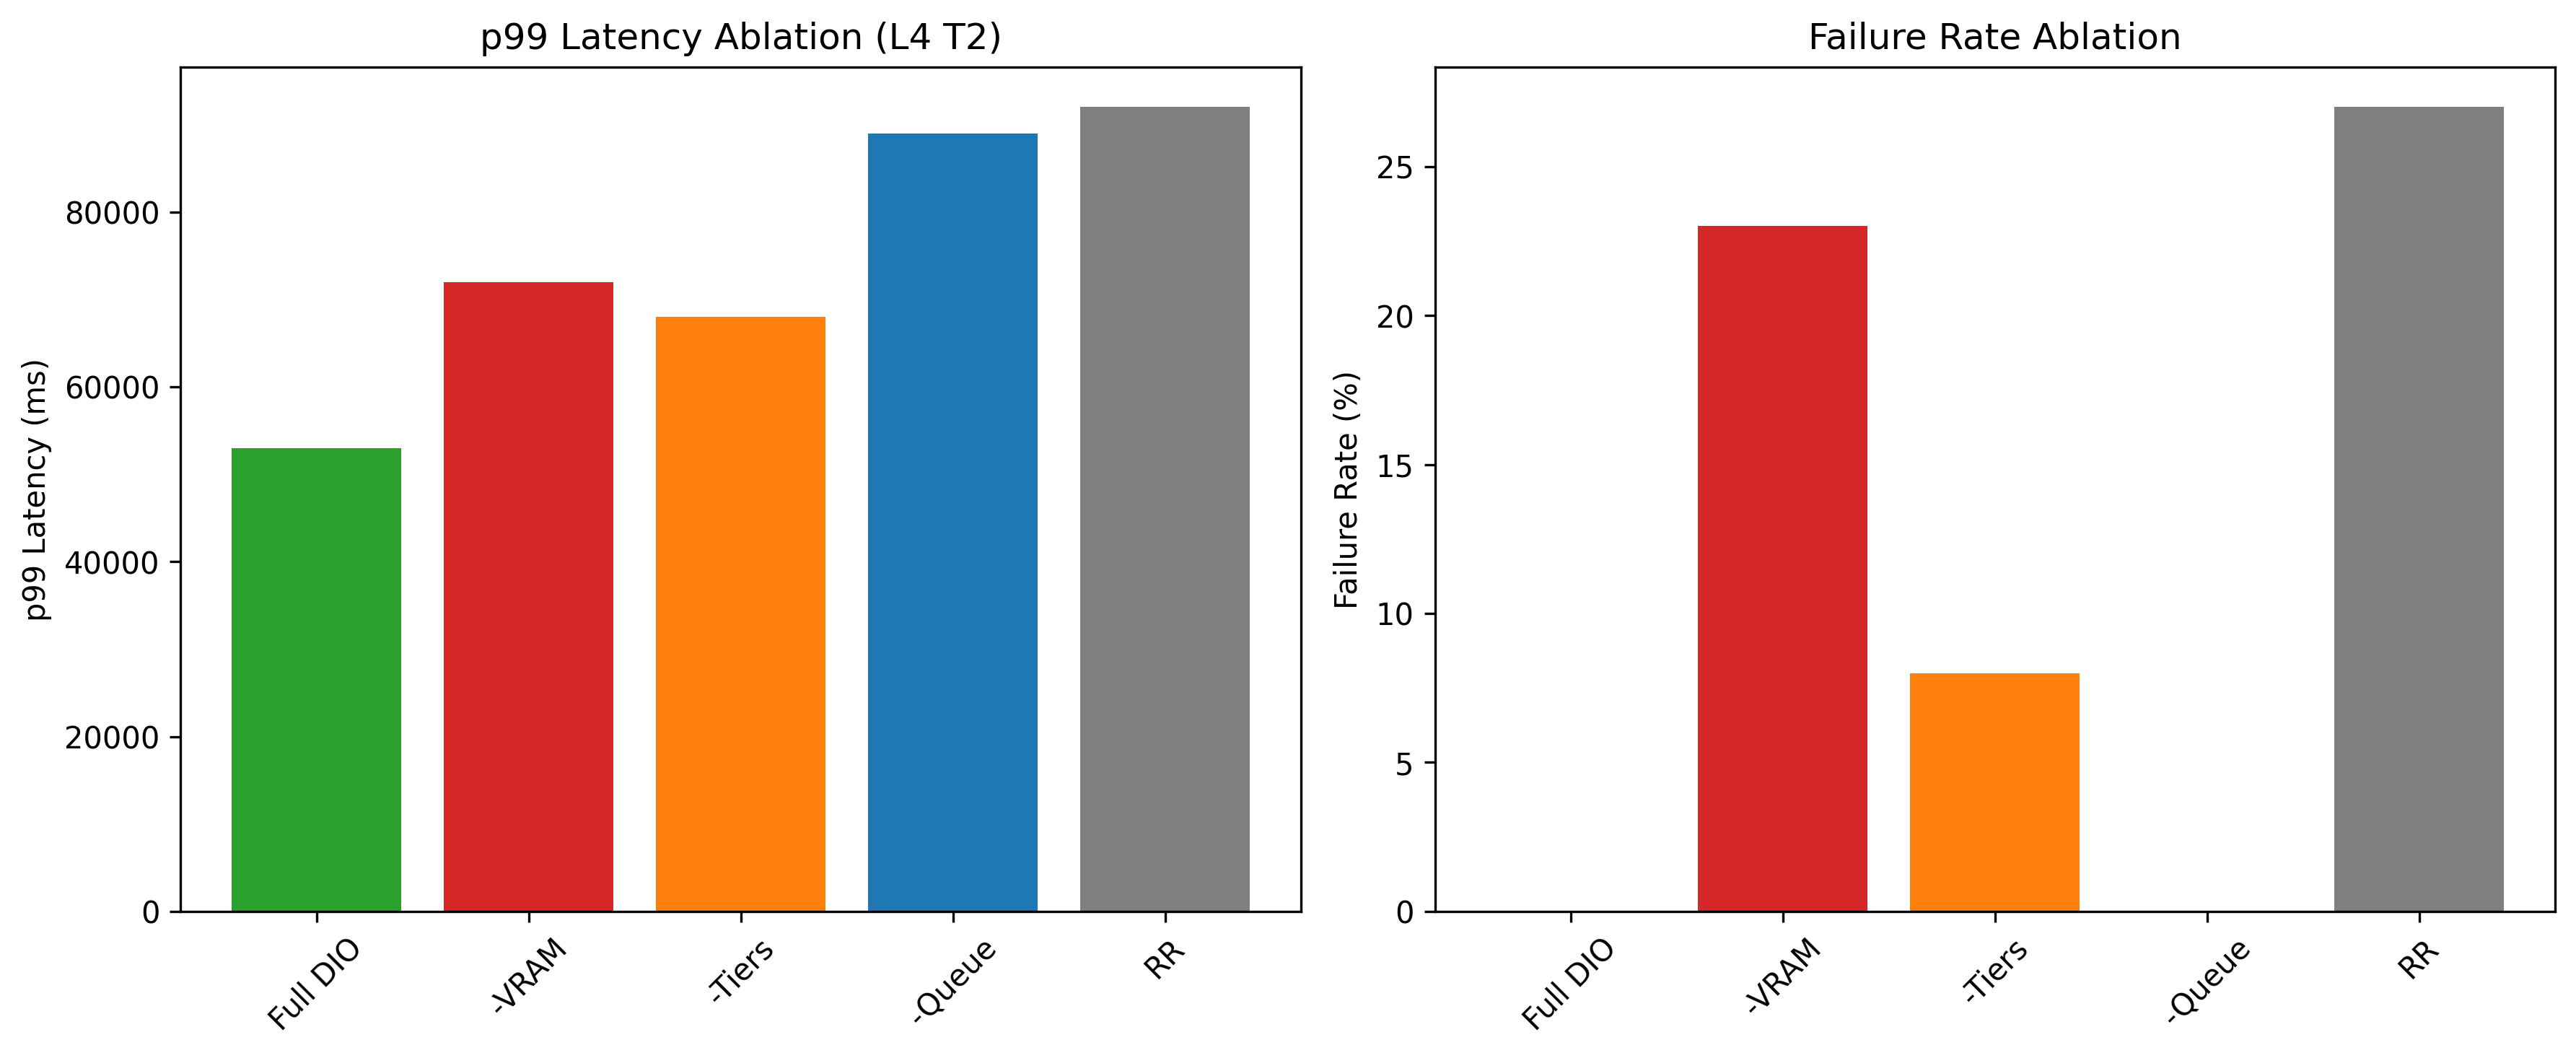
\includegraphics[width=\columnwidth]{fig_ablation.png}
\caption{Cost-term ablation (L4 microbench). Full DIO keeps failures low and tail controlled.}
\label{fig:ablation}
\end{figure}

\begin{figure}[t]
\centering
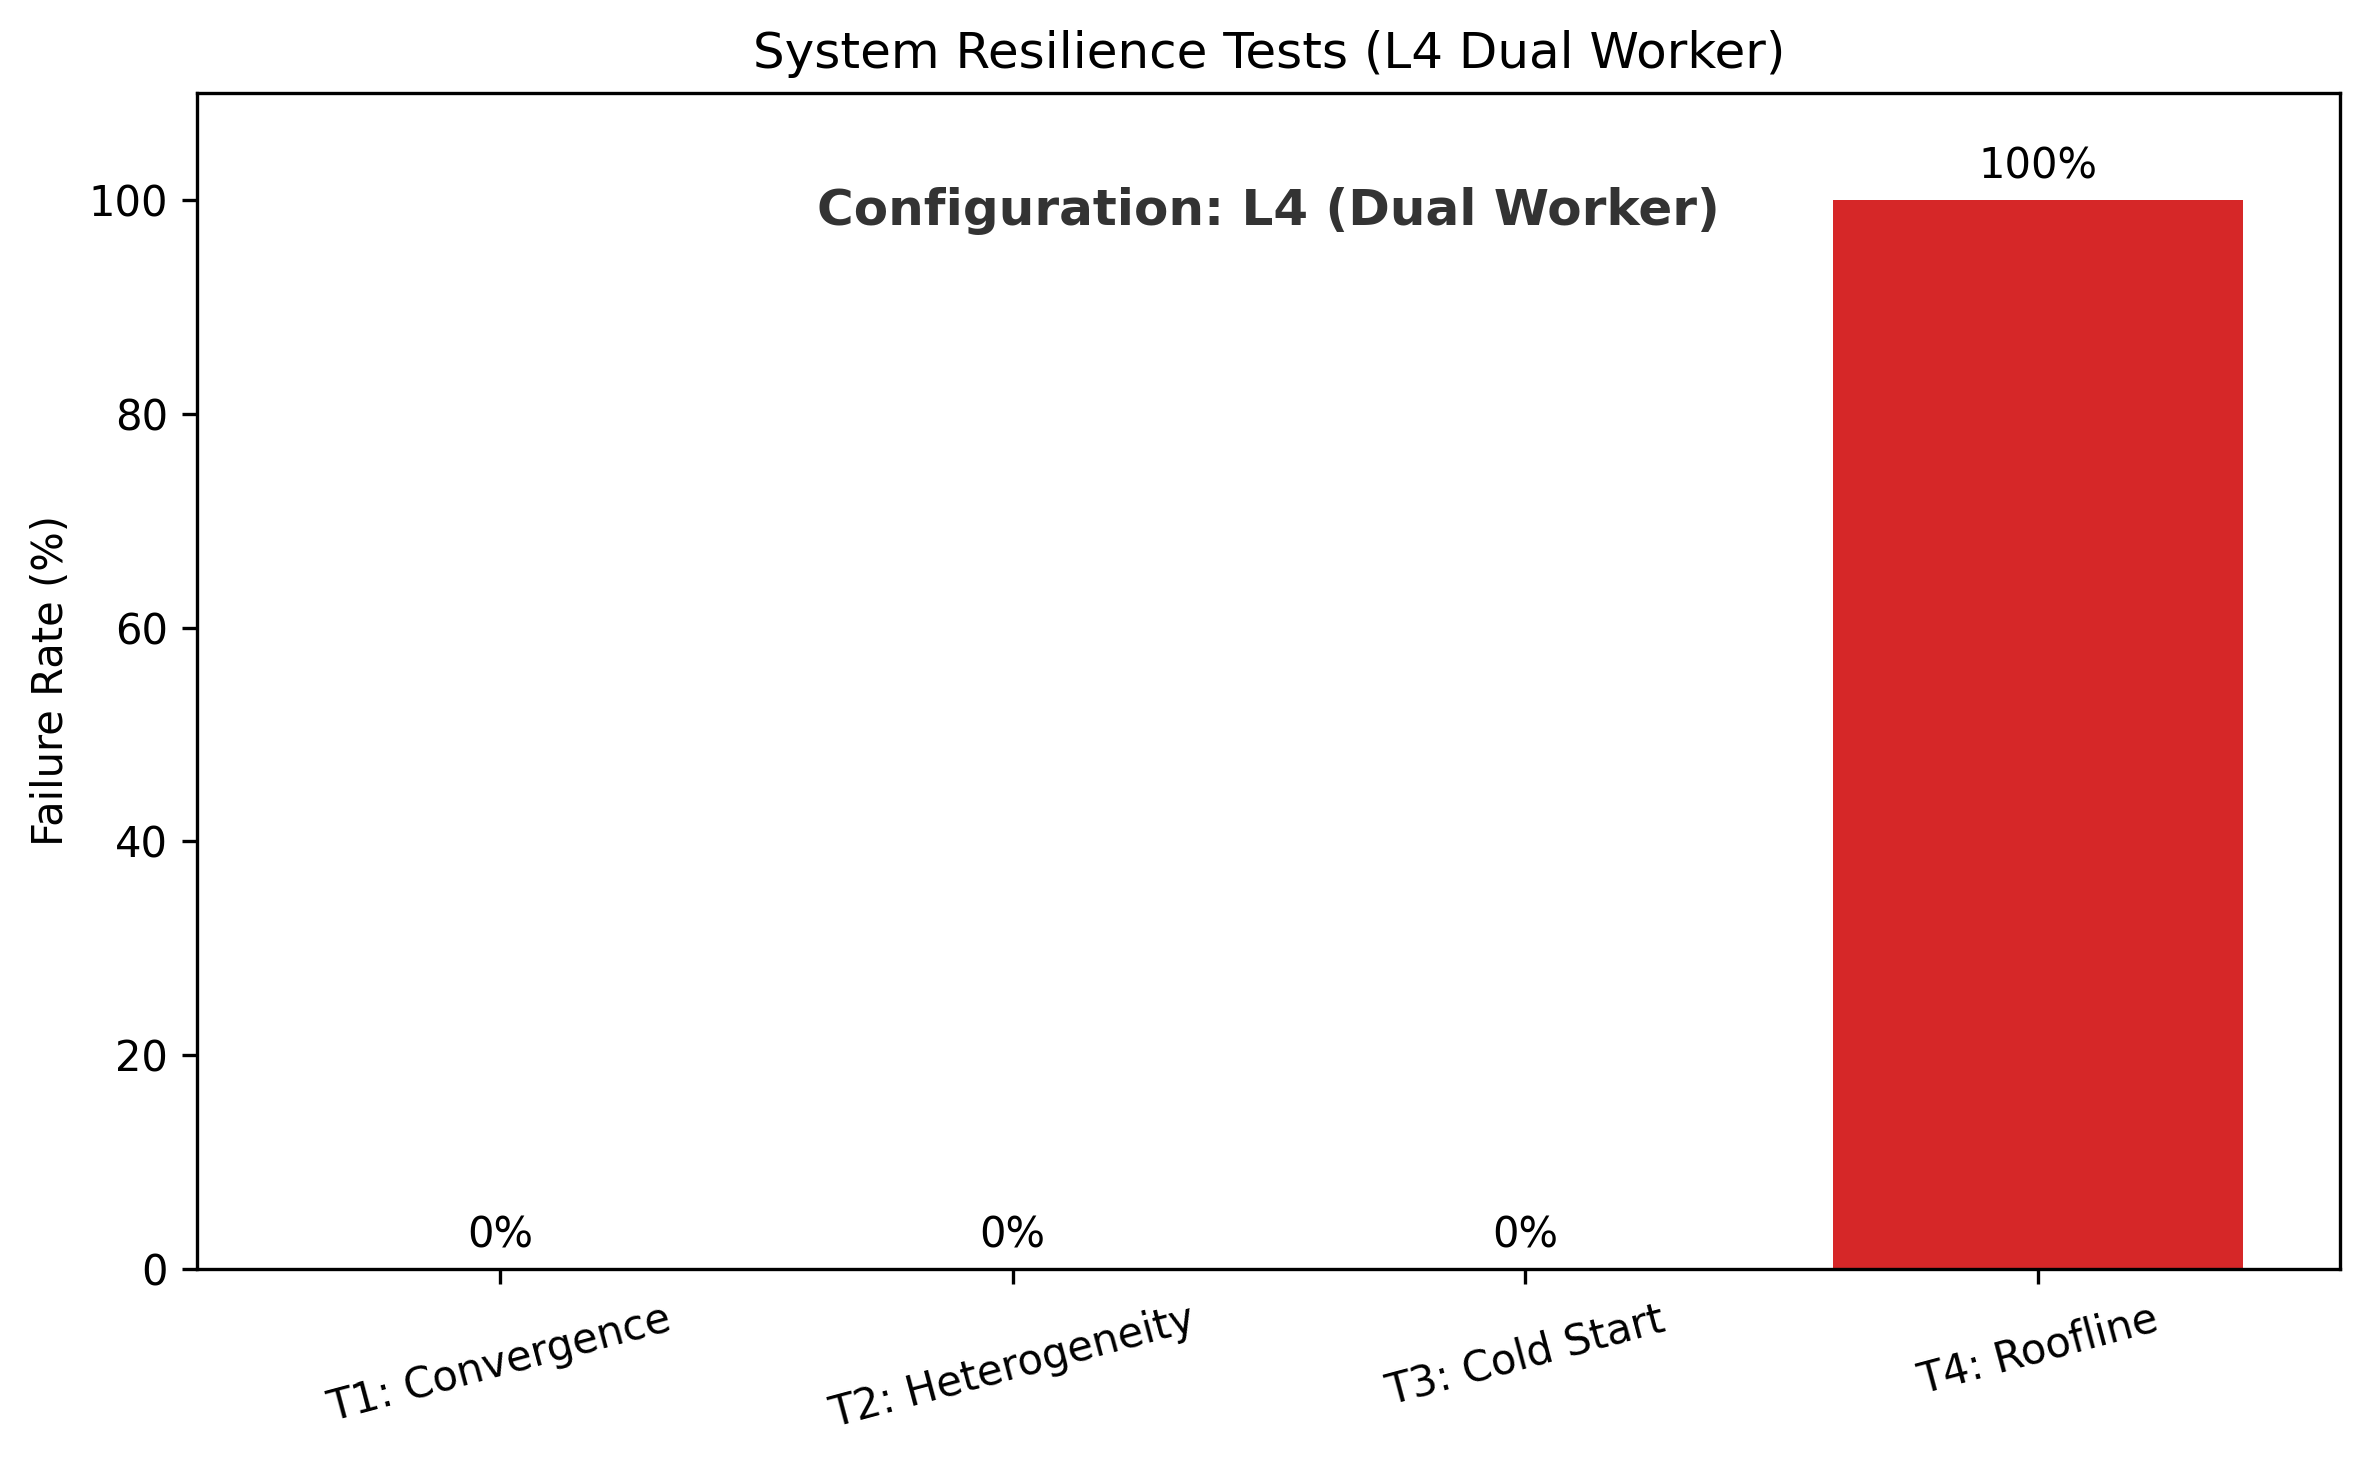
\includegraphics[width=\columnwidth]{fig5_resilience_FINAL.png}
\caption{Resilience microbenchmarks (L4 suite). Overload test exercises admission (503), not throughput maximization.}
\label{fig:resilience}
\end{figure}

%%=============================================================================
\section{Discussion and limitations}
\label{sec:limitations}

\paragraph{Is NLMS ``good at routing''?}
Honestly: \textbf{only when backends differ in observed service cost}---or when hybrid metrics expose pressure that e2e alone has not yet reflected. On matched dual-T4 workers, NLMS alone is no better than RR on mean p99 (Section~\ref{sec:regimeA}). Under a slow peer, NLMS improves p99 substantially vs.\ RR and RLS (Section~\ref{sec:regimeC}). Hybrid scrape terms and session affinity are the complementary answers when the problem is KV/queue pressure or multi-turn cache locality rather than GPU SKU mix. Absolute $\hat{y}$ remains untrustworthy for gating; admission must not assume otherwise.

\paragraph{Limitations.}
\begin{enumerate}
\item \textbf{Telemetry depth.} Hybrid scrape uses what stock vLLM exports; not continuous NVML SM/power/temperature.
\item \textbf{Skew model.} Real GPU skew uses delay-proxy on identical T4s, not physical multi-SKU fleets.
\item \textbf{A/B/C GPU live cells.} Affinity and hybrid p99 gains on live dual-T4 multi-seed under concurrent multi-turn load remain an extension; library suites establish mechanism correctness.
\item \textbf{Baselines.} RR/LL/RLS on the same vLLM pair; not multi-node Orca/vLLM-distributed.
\item \textbf{Workload.} Short sequential chat probes dominate dual-T4 multi-seed cells; concurrent ShareGPT multi-seed is incomplete.
\item \textbf{Out of scope.} Prefill/decode disaggregation co-design, multimodal split inference.
\end{enumerate}

%%=============================================================================
\section{Conclusion}
\label{sec:conclusion}

DIO (\texttt{dio-serve}) is a non-invasive multi-instance gateway for stock vLLM-class engines. We combine (A)~hybrid cost routing---dual-timescale NLMS ranking plus scraped engine KV/queue/prefix metrics---(B)~session/prefix affinity for multi-turn workloads, and (C)~admission control that does not trust absolute $\hat{y}$ when MAPE is high. Multi-seed dual-T4 results show \textbf{no free lunch when backends match} and \textbf{clear p99 gains when one peer is effectively slower}; library suites demonstrate hybrid steering, affinity stickiness, and absolute-vs-empirical admission disagreement. That is a deployable systems contribution for common multi-vLLM deployments---without engine patches, multi-SKU hardware, or full GPU telemetry.

%%=============================================================================
\backmatter

\bmhead{Acknowledgements}
The authors thank colleagues who provided feedback on earlier drafts.

%% Declarations required by Springer Nature journals
\section*{Declarations}

\begin{itemize}
\item \textbf{Funding.} No external funding was received for this work.
\item \textbf{Conflict of interest/Competing interests.} The authors declare that they have no competing interests.
\item \textbf{Ethics approval and consent to participate.} Not applicable (no human subjects or personal data).
\item \textbf{Consent for publication.} Not applicable.
\item \textbf{Data availability.} Aggregated experimental results are included in the repository under \texttt{results\_workshop\_final/} and related result directories. Raw engine logs can be regenerated with the public scripts.
\item \textbf{Materials availability.} Not applicable.
\item \textbf{Code availability.} Source code for \texttt{dio-serve} (including hybrid \texttt{/metrics} scrape, affinity, and admission modes), validation suites (\texttt{run\_workshop\_final\_suite.py}, \texttt{run\_abc\_experiments.py}, delay-proxy harness), and paper artifacts are available in the project repository (\url{https://github.com/nisaral/DIO}).
\item \textbf{Author contribution.} K.N.\ led system design, implementation, experiments, and manuscript drafting. K.P.\ and K.M.\ contributed to evaluation, analysis, and manuscript revision. All authors approved the final manuscript.
\end{itemize}

\begin{appendices}
\section{Notation summary}
\label{app:notation}
\begin{itemize}
\item $s^{\mathrm{fast}}, s^{\mathrm{slow}}, s^{\mathrm{eff}}$: dual-timescale and blended slopes (ms/token).
\item $b_w$: intercept (ms).
\item $N$: token feature; $y$, $\hat{y}$: actual and predicted e2e latency (ms).
\item $S_w$: joint routing cost; $Q_w$: pending queue depth; $B$: batch amortization constant.
\item $\mathrm{KV}_w$, $W_w$, $\mathrm{Hit}_w$: engine-scraped KV usage, waiting requests, prefix hit rate.
\item $c_{\mathrm{kv}}, c_q, c_p$: hybrid cost coefficients (ms scale).
\end{itemize}
\end{appendices}

\bibliography{sn-bibliography}%

\end{document}
